
\begin{frame}{Objectifs du cours}
  Compétences acquises à l'issue de ce cours :
  \begin{itemize}
    \item Concepts derrière l'IA, l'apprentissage automatique
    \item Savoir tirer de l'information d'un jeu de données
    \item Visualiser des données
    \item Mettre en oeuvre les techniques et les appliquer à des cas réels
  \end{itemize}
\end{frame}



\begin{frame}{Programme}

  \begin{columns}
    \begin{column}{0.48\textwidth}
      \begin{tcolorbox}[title=\textsc{\textcolor{black}{Session 1 -- 8 janvier}}, colframe=gray!40]
        \footnotesize{\textbf{Introduction à l'IA\\IA générative}}
      \end{tcolorbox}
    \end{column}

    \begin{column}{.48\textwidth}
      \begin{tcolorbox}[title=\textsc{\textcolor{black}{Session 2 -- 15 janvier}}, colframe=gray!40]
        \footnotesize{Fouille de données \\Visualisation}
      \end{tcolorbox}
    \end{column}
  \end{columns}

  \begin{columns}
    \begin{column}{0.48\textwidth}
      \begin{tcolorbox}[title=\textsc{\textcolor{black}{Session 3 -- 26 janvier}}, colframe=gray!40]
        \footnotesize{Fouille de données textuelles\\}
      \end{tcolorbox}
    \end{column}
    \begin{column}{.48\textwidth}
      \begin{tcolorbox}[title=\textsc{\textcolor{black}{Session 4 -- 29 janvier}}, colframe=gray!40]
        \footnotesize{Eléments d'apprentissage\\automatique}
      \end{tcolorbox}
    \end{column}

  \end{columns}
  
  \bigskip

  \underline{Atelier d'application} : jeudi 5 février, en présentiel

\end{frame}



\begin{frame}{Modalités d'évaluation}

  Les modalités sont les suivantes :

  \begin{enumerate}
    \item Deux travaux seront demandés à l'issue des cours 1 et 2
    \item Mini-projet
    \begin{itemize}
      \item Sur la base de votre projet d'Innovation
      \item Travail en groupe
      \item Fera l'objet de la dernière session en présentiel
    \end{itemize}
  \end{enumerate}

  
\end{frame}


\section{Introduction à \\l'intelligence artificielle}



\begin{frame}{Introduction}
  \begin{center}
      \begin{itemize}
          \item[\textcolor{white}{x}] \textsc{Data science ?}
          \item[\textcolor{white}{x}]
          \item[\textcolor{white}{x}] \textsc{Machine learning ?}
          \item[\textcolor{white}{x}] 
          \item[\textcolor{white}{x}] \textsc{Intelligence Artificielle ?}
      \end{itemize}
  \end{center}
\end{frame}



\begin{frame}{Quelques exemples}
  \begin{center}
    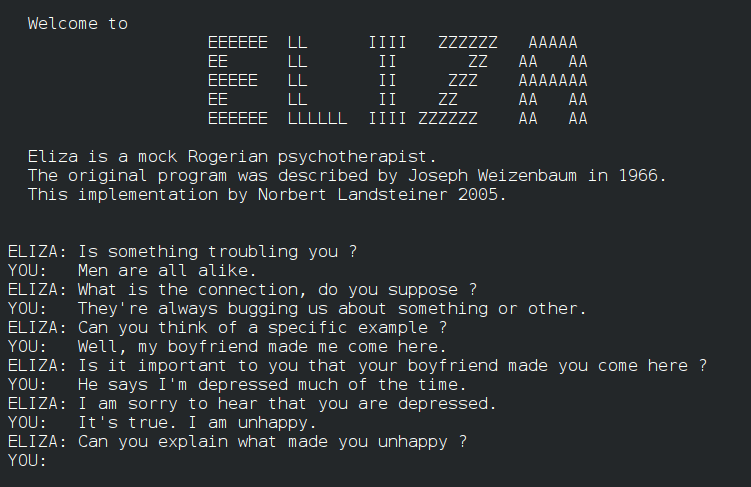
\includegraphics[width=.8\textwidth]{img/intro/eliza.png}

    \Large{1967}
  \end{center}
\end{frame}

\begin{frame}{Quelques exemples}
  \begin{center}
    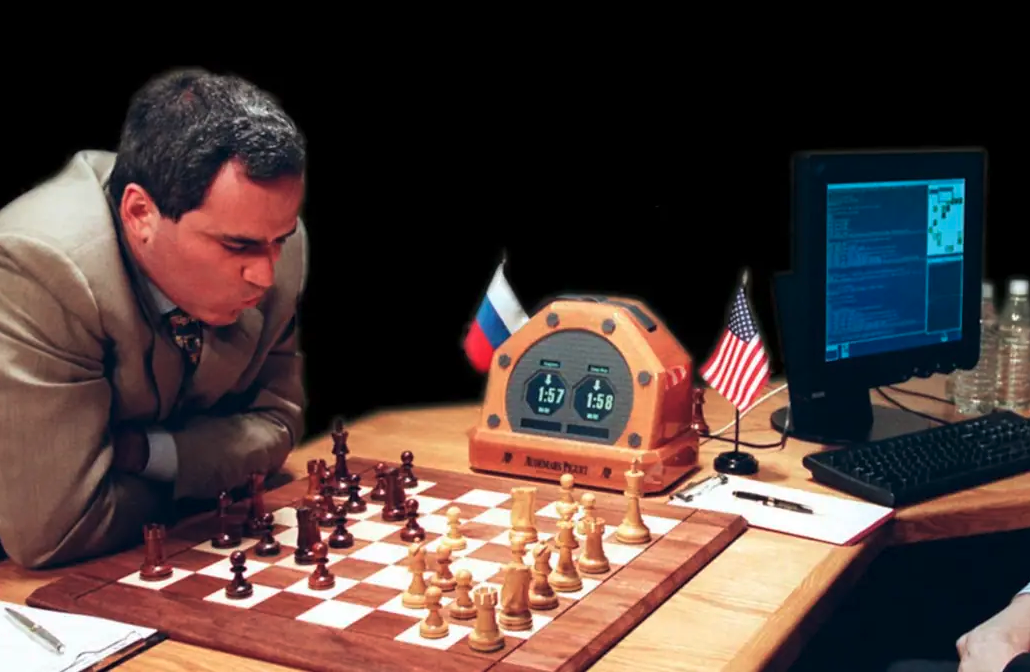
\includegraphics[width=.8\textwidth]{img/intro/deep-blue.png}

    \Large{1996-1997}
  \end{center}
\end{frame}

\begin{frame}{Quelques exemples}
  \begin{center}
    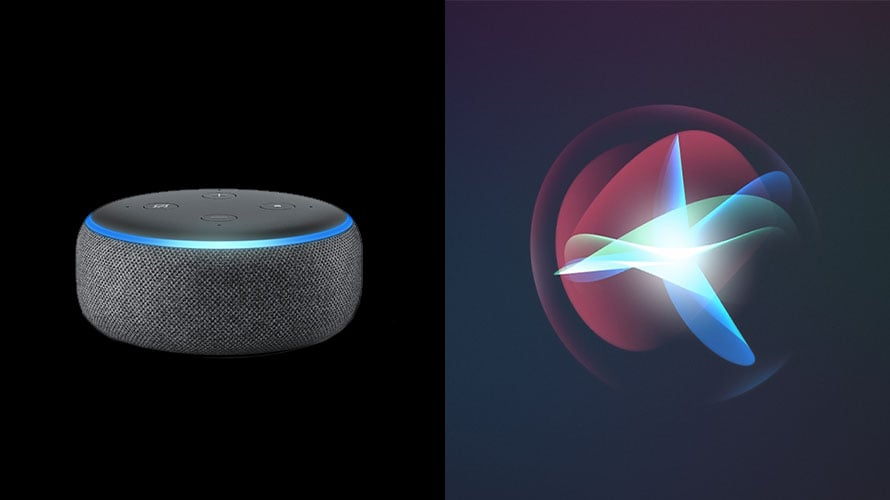
\includegraphics[width=.8\textwidth]{img/intro/siri-alexa.jpg}

    \Large{2014} \hfil  \Large{2011}
  \end{center}
\end{frame}
  
\begin{frame}{Quelques exemples}
  \begin{center}
    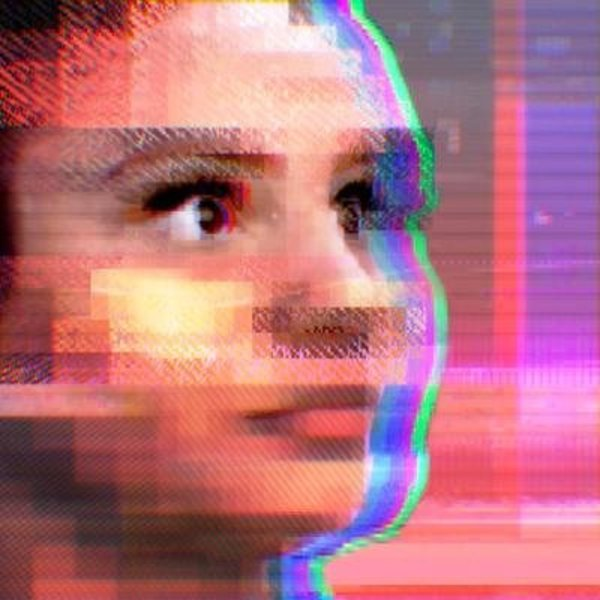
\includegraphics[width=.6\textwidth]{img/intro/tay.jpg}

    \Large{2016}
  \end{center}
\end{frame}

\begin{frame}{Quelques exemples}
  \begin{center}
    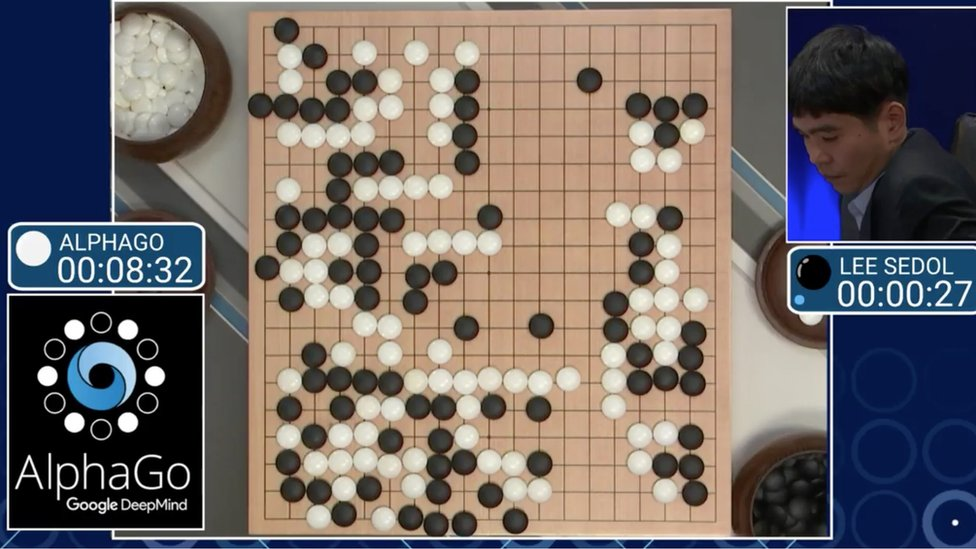
\includegraphics[width=\textwidth]{img/intro/alphago.jpg}
    
    \Large{2016}
  \end{center}
\end{frame}

\begin{frame}{Quelques exemples}
\begin{center}
  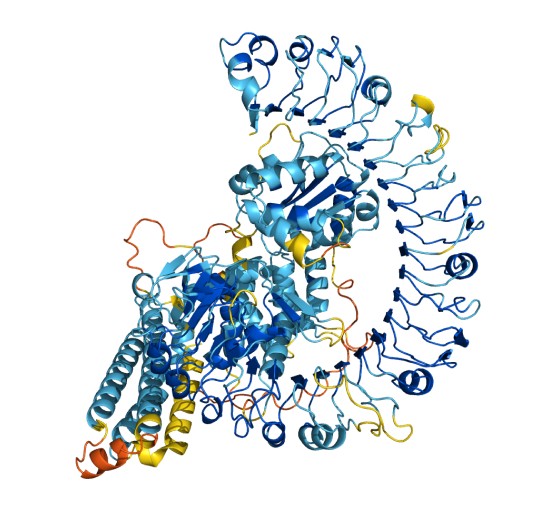
\includegraphics[width=.6\textwidth]{img/intro/alpha-fold.png}
  
  \Large{2018}
\end{center}
\end{frame}



\begin{frame}{Quelques exemples}
  \begin{center}
    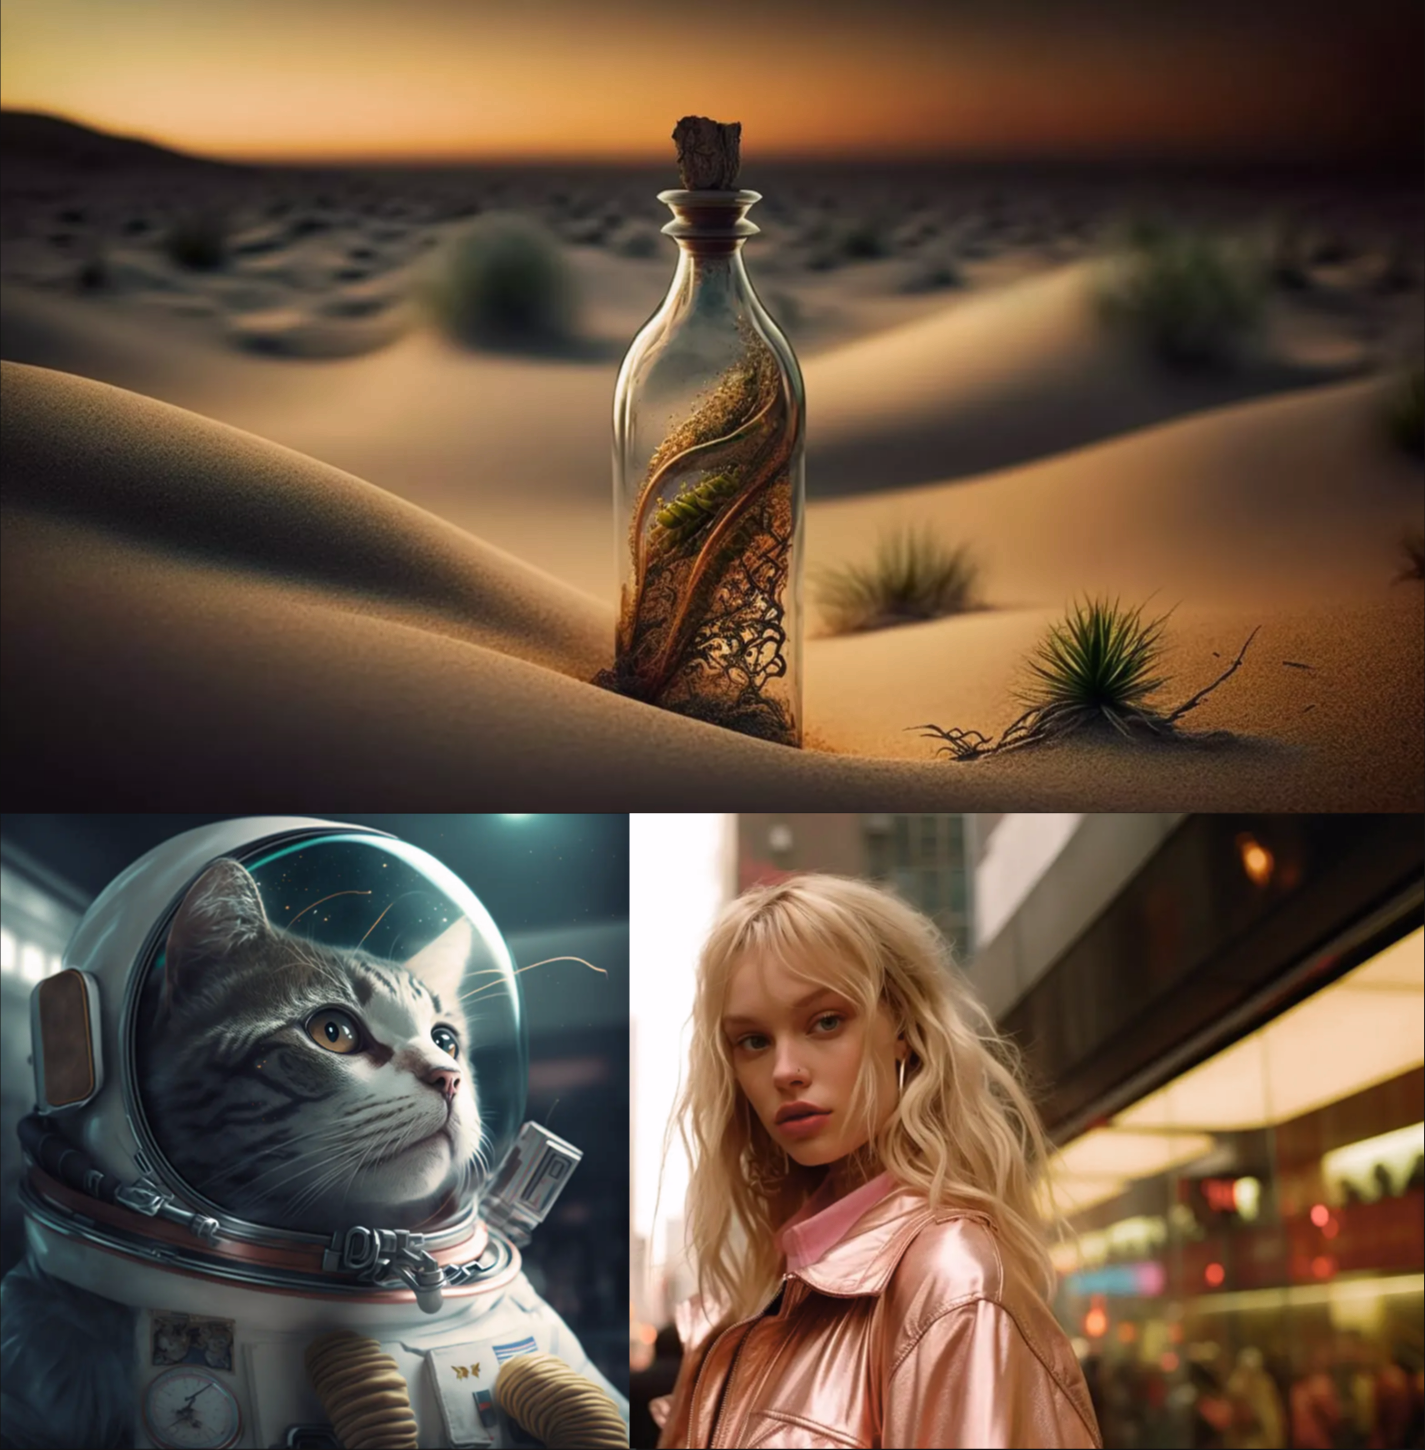
\includegraphics[width=.6\textwidth]{img/intro/midjourney.png}

    \Large{2022-}
  \end{center}
\end{frame}
